%
% ---------- header -----------------------------------------------------------
%
% project       kaneton
%
% license       kaneton
%
% file          /home/mycure/kaneton/view/exam/kernels/2008/nse1/nse1.tex
%
% created       julien quintard   [mon may 14 21:56:41 2007]
% updated       julien quintard   [thu may 22 19:41:38 2008]
%

%
% ---------- setup ------------------------------------------------------------
%

%
% path
%

\def\path{../../../..}

%
% template
%

%%
%% licence       kaneton licence
%%
%% project       kaneton
%%
%% file          /home/mycure/kaneton/view/templates/exam.tex
%%
%% created       julien quintard   [fri dec  2 22:20:57 2005]
%% updated       julien quintard   [mon feb 20 23:01:50 2006]
%%

%
% compile mode
%

%
% ---------- header -----------------------------------------------------------
%
% project       kaneton
%
% license       kaneton
%
% file          /home/mycure/kane...w/talk/presentations/kaneton/kaneton.tex
%
% created       julien quintard   [mon may 14 21:02:29 2007]
% updated       julien quintard   [sun feb  6 20:50:37 2011]
%

%
% ---------- setup ------------------------------------------------------------
%

%
% path
%

\def\path{../../..}

%
% template
%

%
% ---------- header -----------------------------------------------------------
%
% project       kaneton
%
% license       kaneton
%
% file          /home/mycure/kaneton/view/template/talk.tex
%
% created       julien quintard   [wed may 16 18:17:37 2007]
% updated       julien quintard   [fri may 23 19:28:10 2008]
%

%
% ---------- class ------------------------------------------------------------
%

\documentclass[8pt]{beamer}

%
% ---------- common -----------------------------------------------------------
%

\input{\path/package/opk/presentation.tex}


%
% title
%

\title{kaneton}

%
% document
%

\begin{document}

%
% title frame
%

\begin{frame}
  \titlepage
\end{frame}

%
% outline frame
%

\begin{frame}
  \frametitle{Outline}

  \tableofcontents
\end{frame}

%
% ---------- text -------------------------------------------------------------
%


%
% overview
%

\section{Overview}

% 1)

\begin{frame}
  \frametitle{Introduction}

  \term{kaneton} is an educational project intended for students to undertake
  in order to learn about operating system internals.
\end{frame}

% 2)

\begin{frame}
  \frametitle{History}

  \begin{itemize}
    \item[2004]
      \name{Julien Quintard} and \name{Jean-Pascal Billaud} decide
      to introduce an optional low-level programming course to first-year
      enginnering students, now known as \name{kastor};
    \item[2004]
      The course having been well received, \name{SRS - Syst\`emes, R\'eseaux,
      S\'ecurit\'e} students ask them to give such an introductory course the
      same year.
    \item[2005]
      The authorization is given to them to teach a kernel development course
      to \name{SRS} students, from January to October. They therefore decide
      to provide students with the design of a microkernel and let the students
      develop it from scratch, their way. \name{kaneton} is born.
    \item[2006]
      After \name{Jean-Pascal Billaud} fled to \name{VMWare}, \name{Julien
      Quintard} started developing a reference implementation and gave
      students this year a skeleton they had to complete. In addition,
      \name{Cedric Aubouy} and \name{Renaud Lienhart} joined the teaching
      team this year.

      \-

      Besides, the \name{LSE - Laboratoire Syst\`eme EPITA} joined the project
      by putting two students on the development of the \name{kaneton}
      research implementation. \name{Matthieu Bucchianeri} and \name{Renaud
      Voltz} thus joined the project.
  \end{itemize}
\end{frame}


% 3)

\begin{frame}
  \frametitle{History}

  \begin{itemize}
    \item[2007]
      This year, \name{Matthieu Bucchianeri} and \name{Renaud Voltz} took
      over the project for a year by lecturing the course and managing the
      project.

      \-

      \name{Julian Pidancet} and \name{Pierre Duteil} joined the project
      as part of the \name{LSE} but \name{Pierre Duteil} had to leave the
      project. Therefore, \name{Elie Bleton}, who was working at the
      \name{LRDE} before, joined the project.
    \item[2008]
      \name{Julian Pidancet} and \name{Elie Bleton} took over this year
      while \name{Laurent Lec} and \name{Nicolas Grandemange} joined as part
      of the \name{LSE}.

      \-

      At the end of this year, after problems with some students as well as
      conflicts with the \name{LSE}, \name{kaneton} maintainers decided not
      to work with the laboratory anymore.
    \item[2009]
      \name{EPITA} alumni were contacted and joined the educational project
      including \name{Francois Goudal}, \name{Benoit Marcot},
      \name{Enguerrand Raymond}, \name{Jean Guyader} but also
      \name{Fabien Le-Mentec}, an \name{EPITECH} alumnus.
  \end{itemize}
\end{frame}

% 4)

\begin{frame}
  \frametitle{Model}

  The project consists for students to fill in some missing parts of the
  kernel.

  \-

  However, note that, unlike \name{Tiger}, the missing parts will never
  be two lines long.

  \-

  Indeed, in \name{kaneton}, students are asked to implement a feature, say,
  providing memory management. Thus, students are free, in a certain way,
  to implement such a feature as they wish.

  \-

  Since the testing usually consists in verifying that the kernel is able
  to provide the functionality, students should be, most of the time, able
  to implement whatever algorithms \etc{} they wish.
\end{frame}

% 5)

\begin{frame}
  \frametitle{People}

  Let's present the people working on the educational project from where they
  studied to what they are now doing:

  \begin{itemize}
    \item
      \name{Francois Goudal};
    \item
      \name{Benoit Marcot};
    \item
      \name{Jean Guyader};
    \item
      \name{Baptiste Afsa}
    \item
      \name{Louis Vatier}; and
    \item
      \name{Julien Quintard}.
  \end{itemize}
\end{frame}

% 6)

\begin{frame}
  \frametitle{Project}

  \name{kaneton} is an important assignment of the \name{SRS}/\name{GISTR}
  curriculum and, as such, must be taken seriously.

  \-

  Especially, in the last years, \name{EPITA} decided to reduce the duration
  of the project to \term{three} months.

  \-

  As such, the other assignments imposed by the specializations in this
  period have been reduced so that students can focus on \name{kaneton}.
\end{frame}

%
% design
%

\section{Design}

% 1)

\begin{frame}
  \frametitle{Overview}

  The kaneton kernel is very different from the kernels you might be
  familiar with, especially the well-known \name{Windows}, \name{Linux},
  \name{BSD} and so forth.
\end{frame}

% 2)

\begin{frame}
  \frametitle{Microkernel}

  First, kaneton is a microkernel, making it modular from the design
  perspective as well as providing properties such as security.
\end{frame}

% 3)

\begin{frame}
  \frametitle{Distributed Computing}

  kaneton has been designed from the ground up for providing the operarting
  system advanced distributed computing features.
\end{frame}

% 4)

\begin{frame}
  \frametitle{Portability}

  kaneton has been designed with portability in mind, especially through
  a specific portability system that perfectly fits the kernel design.
\end{frame}

% 5)

\begin{frame}
  \frametitle{Organisation}

  Besides being a microkernel, kaneton is well organised in the inside,
  splitting functionalites into objects and managers.
\end{frame}

%
% stages
%

\section{Stages}

% 1)

\begin{frame}
  \frametitle{k0}

  The first project, named \term{k0}, consists for students to learn
  about low-level programming.

  \-

  This project comes with a lecture regarding the boot system as well
  as a practical session.

  \-

  \name{Francois Goudal} will be in charge of this stage which will last for
  a week.
\end{frame}

% 2)

\begin{frame}
  \frametitle{k1}

  \term{k1} consists for students to provide the kaneton microkernel the
  capacity to handle events.

  \-

  During this stage, a lecture on general kernel principles and a lecture on
  interrupts will be taught.

  \-

  \name{Julien Quintard} will be in charge of this stage which will last
  for a single week.

  \-

  Note that, starting with \name{k1}, the student snapshot will be used which
  provide students a development environment, making kernel development easier.
\end{frame}

% 3)

\begin{frame}
  \frametitle{k2}

  \term{k2} consists for students to provide the kaneton microkernel a
  memory management unit so that applications as well as the kernel itself
  can reserve, share \etc{} memory.

  \-

  During this stage, a lecture on portability as well as lectures on
  memory management will be taught.

  \-

  \name{Francois Goudal} will be in charge of this stage which will last
  for three weeks.
\end{frame}

% 4)

\begin{frame}
  \frametitle{k3}

  In \term{k3}, students will have to provide kaneton with execution contexts
  such that the kernel can execute multiple threads at the \textit{same} time.

  \-

  Lectures, during this stage, will discuss topics such as interrupts,
  concurrency, multi-processing, scheduling \etc{}

  \-

  \name{Benoit Marcot} will be in charge of this stage which will last for
  three weeks.
\end{frame}

% 5)

\begin{frame}
  \frametitle{Evaluation}

  For every stage, students will have the possibility to test their
  implementation by running, a limited number of times, the test suite used
  for evaluating their work.

  \-

  Besides, at the end of each stage, after submission, the kaneton test system
  will run the test suite and issue a mark according to the test results.

  \-

  Additionally, an exam will take place at the end of the semester to make
  sure that the notions tackled throughout the course are well understood
  by every student.
\end{frame}

%
% tools
%

\section{Tools}

% 1)

\begin{frame}
  \frametitle{Overview}

  The kaneton educational project relies on tools, sometimes developed
  internally.
\end{frame}

% 2)

\begin{frame}
  \frametitle{Web Site}

  The web site contains the documentation including design papers,
  the assignments \etc{} but also hosts the wiki which should be
  the starting point for every student seeking information.

  \-

  Noteworthy is that the wiki contains courses regarding the
  inline assembly, linking, pre-processing and so on. Students
  are invited to read them all as they will come handy when
  developing the kaneton stages.

  \-

  \name{Julien Quintard} should be contacted for requests regarding the
  web site and wiki.
\end{frame}

% 3)

\begin{frame}
  \frametitle{Snapshot}

  The student snapshot has been automatically generated from the current
  kaneton implementation.

  \-

  \name{Francois Goudal} is in charge of this process, hence should be
  contacted if you believe there is a mistake.
\end{frame}

% 4)

\begin{frame}
  \frametitle{Cheat}

  Every student's kaneton implementation will be tested to make sure that
  students did not cheat by relying on implementations by previous or
  current students.

  \-

  \name{Julien Quintard} is in charge of this tool.
\end{frame}

% 5)

\begin{frame}
  \frametitle{Test}

  Students' implementation will be tested in a real environment by applying
  a complete test suite; hence, validating the implementation's behaviour.

  \-

  \name{Jean Guyader} is responsible of this tool and should be contacted
  if necessary.
\end{frame}

%
% information
%

\section{Information}

% 1)

\begin{frame}
  \frametitle{Support}

  \begin{enumerate}
    \item
      \term{Website}

      \-

      You will find on \location{http://kaneton.opaak.org} documents regarding
      the project from the design to the implementation;
    \item
      \term{Wiki}

      \-

      The wiki \location{http://wiki.opaak.org} is the best way to get
      technical information as well as to help other students by adding
      and/or improving pages' contents;
    \item
      \term{Mailing-List}

      \-

      The kaneton educational students mailing-list
      \location{students@kaneton.opaak.org} will be used by teachers as
      an official means for communicating with students.

      \-

      Therefore, every student should subscribe to this mailing-list by sending
      an email to \location{students+subscribe@kaneton.opaak.org}.

      \-

      It is not allowed to post code on the mailing list, or give pointers to
      code in the snapshot that would provide obvious solution to somebody's
      question.
  \end{enumerate}
\end{frame}

% 2)

\begin{frame}
  \frametitle{Groups}

  Except for \name{k0} which is an individual project, the other projects
  from \name{k1} to \name{k3} are done in groups of \term{two} students.

  \-

  Every group is expected to send an email to
  \location{admin@opaak.org}.

  \-

  Note that we will use students' \name{EPITA} email addresses. As such,
  make sure that you check this email box.
\end{frame}

% 3)

\begin{frame}
  \frametitle{Reliance}

  As for \name{Tiger}, every stage depends on the previous one, except
  for \name{k0}.

  \-

  As such, test suites from the previous stages will also be used for both
  testing and marking.

  \-

  Students should therefore make sure to use their test permissions for making
  sure to fix the bugs of previous stages so that such bugs do not impact
  on the current stage results, hence mark.
\end{frame}

% 4)

\begin{frame}
  \frametitle{Machine}

  This year, the machine used by the kaneton educational project will consists
  of the \term{IBM-PC} platform coupled with the \term{IA-32} microprocessor
  architecture \ie{} the most common hardware system on the market.

  \-

  Although it is always best to test your implementation on a real machine,
  it takes time to reboot a real computer. You should therefore use an
  emulator such a \name{QEMU} or \name{Bochs} as they will enable you to
  test your kernel very quickly but they will also let you develop on
  a non-\name{IBM-PC}/\name{IA-32} machine such as a \name{Mac} for example.
\end{frame}

%
% conclusion
%

\section{Conclusion}

% 1)

\begin{frame}
  \frametitle{Concepts}

  Throughout the project, you will learn so many things from terminology,
  to how a computer boots, how the kernel controls the hardware and how it
  provides abstractions as basic as execution contexts.

  \-

  At the end of the project, you will definitely know that nothing is magic
  but purely logic and often actually very simple.
\end{frame}

% 2)

\begin{frame}
  \frametitle{Implementation}

  Although, starting the project by learning how to make a computer execute
  your code, you will end up, after three months, with a running kernel
  and operating system capable of executing programs, the whole on real
  hardware like the machine you have at home.
\end{frame}

% 3)

\begin{frame}
  \frametitle{Changes}

  Over the years, the project has greatly evolved, from a no-implementation
  project, to a reference-based project.

  \-

  However, being a project developed by volunteers willing to dedicate some
  time so that other students can learn, many things are missing and/or
  can be improved including the lectures but also the project implementation.

  \-

  In conclusion, keep in mind that the project exists only because of people
  willing to transfer their knowledge and please respect their effort.
\end{frame}

% 4)

\begin{frame}
  \frametitle{Fun}

  But most of all, kaneton should be about learning through fun!
\end{frame}

% 5)

\begin{frame}
  \frametitle{Reminder}

  Remember to perform the following tasks:

  \begin{itemize}
    \item
      Send an email to \location{admin@opaak.org} regarding the composition
      of your group, before \textbf{Wednesday 16th 2pm} or you will be put
      in a group by force;
    \item
      Subscribe to the students mailing-list
      \location{students@kaneton.opaak.org} by sending an email to
      \location{students+subscribe@kaneton.opaak.org};
    \item
      Watch closely the \name{Wiki} at \location{http://wiki.opaak.org} by
      subscribing the \name{RSS} feed for example;
    \item
      We advise SRS/GISTR lab roots to set up a \name{Xen}-based environment
      as testing on emulators only will become difficult over time;
    \item
      Students must have a ``rack'' containing a \name{POSIX}-compilant
      operating system for the \name{k0} practical session.
  \end{itemize}
\end{frame}

\end{document}


%
% class
%

\documentclass[10pt,a4wide]{article}

%
% packages
%

\usepackage[english]{babel}
\usepackage[T1]{fontenc}
\usepackage{a4wide}
\usepackage{graphicx}
\usepackage{fancyheadings}
\usepackage{multicol}
\usepackage{indentfirst}
\usepackage{color}
\usepackage{ifthen}
\usepackage{comment}
\usepackage{verbatim}
\usepackage{aeguill}

\pagestyle{fancy}

\setlength{\footrulewidth}{0.3pt}
\setlength{\parindent}{0.3cm}
\setlength{\parskip}{2ex plus 0.5ex minus 0.2ex}

%
% correction environment
%

\newenvironment{correction}%
   {
     \ifthenelse
	 {
	   \equal{\kaneton-latex}{subject}
	 }
	 {
	   \comment
	 }
	 {
	   \textbf{\color{red}{ ----- correction}}
	 }
   }%
   {
     \ifthenelse
	 {
	   \equal{\kaneton-latex}{subject}
	 }
	 {
	   \endcomment
	 }
	 {
	   \textbf{\color{red}{ ----- /correction}}
	 }
   }

%
% header
%

\rfoot{\scriptsize{Exam}}

\date{\scriptsize{\today}}


%
% listings package
%

\usepackage{listings}
\definecolor{darkgray}{rgb}{0.95,0.95,0.95}
\lstset{language=C}
\lstset{backgroundcolor=\color{darkgray}}
\lstset{numbers=left, numberstyle=\tiny, tabsize=4, stepnumber=1, numbersep=5pt}
\lstset{keywordstyle=\bfseries}
\lstset{basicstyle=\footnotesize}

\setlength{\marginparwidth}{10pt}
%
% header
%

% \lhead{\scriptsize{Noyaux et Syst\`emes d'exploitation}}
% \rhead{\scriptsize{2008}}

%
% title
%

\title{{\huge {\bf Noyaux et Syst�mes d'exploitation}}}

%
% authors
%

\author{{Julian Pidancet \& Elie Bleton}}

%
% document
%

\begin{document}

%
% title
%

\maketitle

%
% identation
%

\indentation{}

%
% --------- information -------------------------------------------------------
%

\begin{center}
\vspace{1cm}

{\huge {\bf Examen NSE1}}

\vspace{2cm}

{\large
{\bf Ordinateurs, PDA et t�l�phones non autoris�s}

{\bf Documents autoris�s}

\vspace{1cm}

{\bf Dur�e : 2 heures}
}
\end{center}

\vspace{2cm}

{\large {\bf Important :}}\\
\begin{itemize}
\item Le bar�me est donn� � titre indicatif, en cas de modifications,
      aucune contestation ne sera possible.

\item Un point de malus sur la note globale sanctionnera les copies peu
      soign�es ou mal orthographi�es.

\item Vos r�ponses seront concises : {\bf courtes, claires et pr�cises}.

\item Lorsqu'il vous est demand� d'�crire du code vous pourrez
     n�gliger la gestion des erreurs uniquement lorsqu'elle
     n'apporte rien au probl�me. En revanche, vous devrez g�rer les
     erreurs provoquant un segfault.
\end{itemize}


%
% --------- text --------------------------------------------------------------
%

\vspace{3cm}

\newpage
\part*{Exercices}

\section*{Exercice 1 : Assembleur (3 points)}

Le code assembleur suivant est execut� sur un microprocesseur Intel
80386 en mode r�el.

Indiquez, pour chaque instruction, ce qu'elle fait.

\begin{verbatim}
MOV AX, 0x1200
MOV ES, AX
MOV BX, 0x4000
MOV AL, [ES:BX]
TEST AL, AL
JZ end
ADD AL, 42
MOV AH, 0xE
INT 0x10
\end{verbatim}


\newpage

\section*{Exercice 2 : Allocation M�moire (6 points)}

SunOS 5.4 introduit en 1994 un nouveau type d'allocateur m�moire grain fin
appel� ``slab allocator''.

Des allocateurs m�moire similaires ont ensuite �t� impl�ment�s dans Linux,
FreeBSD et beaucoup d'autres syst�mes d'exploitations.

Le principe de l'allocateur se base sur plusieurs hypoth�ses :
\begin{itemize}
  \item Les blocs de m�moire allou�s par l'utilisateur sont souvent de
        taille identique. Car la plupart du temps, ceux-ci correspondent
	a des objets pour le noyau.
  \item Lors de la lib�ration d'un objet, la lib�ration de la m�moire physique
        correspondante est pr�matur�e. Un comportement de cache est pr�f�rable.
  \item La gestion des structures internes de l'allocateur ne doit pas �tre
	plus lourde que l'allocation m�moire elle-m\^eme.
\end{itemize}

Cet allocateur est compos� d'objets appel�s ``caches'' et ``slabs''.
Un cache maintient une liste de slabs qu'il g�re. Un slab contient
physiquement un ensemble de blocs m�moire de taille identique.

Dans notre noyau exp�rimental chicheOS, nous disposons du code suivant :

\begin{verbatim}

/* Objet cache */
typedef struct
{
  kmem_slab_t   *slab_list;     /* Liste de slabs du cache */
  kmem_slab_t   *free_slab;     /* Pointe vers un slab qui contient au moins
                                   un bloc libre */

  size_t	obj_size;       /* Taille des objets stockes dans les slabs du
                                   cache */

  ...

} kmem_cache_t;

/* Descripteur de slab */
typedef struct
{
  int           nobjs_max;      /* Nombre de blocs contenus dans le slabs */
  int           nobjs;          /* Nombre de blocs alloues */

  int		first_free;	/* Index d'un bloc libre */

  char*         block_list;	/* Pointe vers la liste des blocs m�moire */
  int*		free_list;	/* Tableau d'entiers contenant pour chaque bloc :
                                   -1 si le bloc est deja allou�
                                   l'index d'un autre bloc libre si le bloc
				     est libre */

  kmem_slab_t   *next;          /* Liste doublement chain�e circulaire des */
  kmem_slab_t   *prev;          /* slabs du cache */

  kmem_cache_t  *cache;         /* Pointeur vers le cache qui possede ce slab */

} kmem_slab_t;

\end{verbatim}

On suppose que chaque slab occupe exactement 1 page m�moire de 4096 octets :

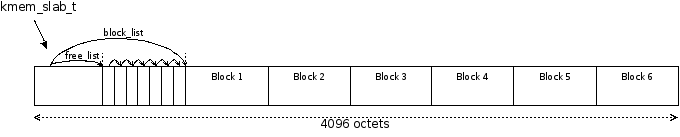
\includegraphics[width=\textwidth]{figures/slablayout.png}

\subsection*{Questions}

\begin{enumerate}
\item Vous disposez de \verb+kmem_cache_t * kmem_cache_region+, un pointeur vers
le cache qui g�re tout les objets de type \verb+region_t+.  Ecrivez la fonction
\verb+region_t * kmem_region_alloc()+ qui alloue un objet
\verb+region_t+ en m�moire. (Vous ne devez pas g�rer le cas d'ajout d'un slab dans le cache)
\item On souhaite lib�rer un objet \verb+region_t+ allou� pr�alablement par la fonction
\verb+kmem_region_alloc()+. Proposez une solution simple pour retrouver le slab
dans lequel se situe notre objet, \`a partir de son adresse.
\item Quels types d'objets ne peuvent pas �tre allou� le slab allocator de ChicheOS ?
\item ChicheOS est �crit en C, n�ammoins, on souhaite pouvoir initialiser et nettoyer
le contenu des objets \verb+region_t+ lors de leur allocation et lib�ration.
Comment peut-on s'y prendre ?
\end{enumerate}



\newpage

\section*{Exercice 1 : M\'ecanisme d'interruptions (3 points)}

{\bf C\^ot\'e microprocesseur}

\begin{enumerate}
\item Comparez les deux diff\'erentes mani\`eres choisies pour les architectures MIPS et IA32 pour permettre au noyau de s\'electionner une ISR sp\'ecifique pour chaque interruption.
\item D\'etaillez le m\'ecanisme mis en oeuvre par le microprocesseur lors du d\'eclenchement d'une interruption mat\'erielle ET du retour vers la t\^ache interrompue.

\begin{itemize}
\item Ne d\'etaillez pas le fonctionnement interne du contr\^oleur d'interruption
\item La t\^ache interrompue s'ex\'ecute en Userland
\item Vous formulerez votre r\'eponse sous la forme d'une liste ordonnant les op\'erations effectu\'ees par le microprocesseur de mani\`ere chronologique.
\end{itemize}

\end{enumerate}



\newpage

\section*{Exercice 4 : Pagination (6 points)}

Nous souhaitons d�velopper un syst�me de gestion de la m�moire
virtuelle pour ChicheOS sur l'architecture Intel. Trois mots d�crivent
la philosophie de ChicheOS : ``maintenir, r�parer et pr�voir''. En
cons�quence, ChicheOS �vite avec prudence la p�rilleuse technique du
\textit{mirroring}.

Le noyau ChicheOS doit pouvoir acc�der \`a n'importe quelle adresse
physique par le biais de traductions d'adresses temporaires, tout en
optimisant l'utilisation du TLB \footnote{\emph{Rappel:} Translation
  Lookaside Buffer : cache de traduction d'adresse}.

Afin de permettre la mise en place de traductions temporaires,
ChicheOS rend accessible une table de page particuli�re depuis
l'espace d'adressage du noyau. Cette table de page particuli�re est
nomm�e CPT \footnote{Chiche Page Table}. \textup{La CPT est utilis�e
  comme un \textbf{cache} de traduction d'adresses}.

\begin{itemize}
\item La CPT se situe en m�moire physique \`a l'adresse physique
  \verb+0x100b000+.
\item La CPT est accessible dans l'espace d'adressage du
  noyau \`a l'adresse \verb+0xC0000000+.
\item L'entr�e num�ro \verb+0x380+
  du Page Directory du noyau contient l'adresse physique de la CPT.
\end{itemize}

\subsection*{API ChicheOS}
\begin{itemize}
\item \verb+int rand_1024()+ : Renvoie un nombre al�atoire
  entre 0 et 1023 inclus.
\item \verb+void pt_entry(int entry, vaddr_t pt, paddr_t page)+ : Ajoute
  une entr�e dans une Page Table \`a l'index \verb+entry+ et ajuste les
  param�tres de l'entr�e de mani�re \`a cr�er une
  translation d'adresse privil�gi�e valide pour le noyau.
\item \verb+char get_entry_data(int entry, vaddr_t pt)+ : Retourne les 3
  bits du champ AVL d'une entr�e de Page Table. Les sp�cifications Intel
  documentent ces 3 bits comme ``Available for programmer use''.
\item \verb+void set_entry_data(int entry, vaddr_t pt, char data)+ :
  Ecris les 3 bits du champs AVL d'une entr�e de Page Table avec la valeur
  des 3 bits de poid faible de \verb+data+.
\end{itemize}

\subsection*{Questions}

\begin{enumerate}
\item Quelle quantit� au total de m�moire virtuelle est rendue
  accessible par notre cache ?

\item \`A quelles adresses (en m�moire virtuelle) est-il possible
  d'acc�der aux traductions contenues par la Page Table ?

\item Si la CPT est pleine\footnote{Toutes les traductions possibles
    sont fa\^ites}, l'ajout d'une nouvelle entr�e suppose la
  suppression d'une vieille entr�e. Pour d�terminer l'entr�e du cache
  a retirer, �crivez une fonction impl�mentant un des algorithmes de
  remplacement d'entr�es vu en cours (LRU, NFU ...). \footnote{Si vous
    s�chez, vous pouvez utiliser la fonction rand\_1024()}

\item �crivez la fonction
  \verb+vaddr_t cache_get_mapping(paddr_t phys)+. Cette fonction
  retourne l'adresse virtuelle d'une traduction vers \verb+phys+ si la
  traduction existe d�j�, ou cr�e la traduction dans le cache le cas
  �ch�ant.

\item Expliquez comment on peut fabriquer un espace d'adressage
  utilisateur \`a partir de z�ro en utilisant la fonction
  \verb+cache_get_mapping()+ et une fonction
  \verb+paddr_t get_physical_page()+ qui alloue des pages de m�moire
  physique.
\end{enumerate}



\end{document}
